\documentclass[a4paper, 12pt]{article}

\usepackage{mathtext}
\usepackage{amsmath}
\usepackage[utf8]{inputenc}
\usepackage[english,russian]{babel}
\usepackage{graphicx, float}
\usepackage{tabularx, colortbl}
\usepackage{caption}
\usepackage{textcomp}
\captionsetup{labelsep=period}

\newcommand{\parag}[1]{\paragraph*{#1:}}
\DeclareSymbolFont{T2Aletters}{T2A}{cmr}{m}{it}
\newcounter{Points}
\setcounter{Points}{1}
\newcommand{\point}{\arabic{Points}. \addtocounter{Points}{1}}
\newcolumntype{C}{>{\centering\arraybackslash}X}

\author{Калинин Даниил, Б01-110}
\date{07.09.2021}
\title{Лабораторная работа 1.1.1. Определение систематических и случайных погрешностей при измерении удельного сопротивления нихромовой проволоки}

\begin{document}
\maketitle

\parag {Цель работы}
измерить удельное сопротивление проволоки и вычислить систематические и случайные погрешности при использовании таких измерительных приборов, как линейка, штангенциркуль, микрометр, амперметр, вольтметр, мост постоянного тока.

\parag {В работе используются}
проволока из нихрома, линейка, штангенциркуль, микрометр, амперметр, вольтметр и мост постоянного тока, источник ЭДС, ключ и реостат.

\parag {Теоритическая справка} ~\\
Удельное сопротивление материала проволоки круглого сечения, изготовленной из одного материала и имеющей одну толщину, может быть определено по формуле:

\begin{equation} \label{eq:1}
    \rho = \frac{R_{пр}}{l}  \frac{\pi d^2}{4}
\end{equation}

Где $R_{пр}$    -- сопротивление измеряемого участка проволоки,
    $l$         -- длина измеряемого участка проволоки,
    $d$         -- диаметр проволоки.

Пусть $V$ и $I$ -- показания вольтметра и амперметра в каждой схеме соответственно. Тогда для схем (а) и (б) соответственно, сопротивление участка проволоки можно вычислить по следующим формулам:

Для схемы (а):
\begin{equation} \label{eq:2}
    R_{пр} =  R_{пр1} (1 + \frac{R_{пр1}}{R_{V}})
\end{equation}

Для схемы (б):
\begin{equation} \label{eq:3}
    R_{пр} =  R_{пр2} (1 - \frac{R_{A}}{R_{пр2}})
\end{equation}

Где $R_{пр1} = \frac{V_a}{I_a}$ -- сопротивление рассчитанное по       показаниям приборов в схеме (а),
    $R_{пр2} = \frac{V_б}{I_б}$ -- сопротивление рассчитанное по       показаниям приборов в схеме (б),
    $R_V$ -- сопротивление вольтметра,
    $R_A$ -- сопротивление амперметра.

\parag {Ход работы} ~\\
Точность измерения с помощью штангенциркуля -- 0.1 мм., Точность измерения с помощью микрометра -- 0.01 мм.\\

\point Измеряем диаметр проволоки штангенциркулем ($d_1$), и микрометром ($d_2$) на 10 различных участках, результат занесем в таблицу \ref{tabl:diam}.

\begin{table}[h!]
    \centering
    \begin{tabular}{|c|c|c|c|c|c|c|c|c|c|c|}
        \hline
        & \textbf{1} & \textbf{2} & \textbf{3} & \textbf{4} & \textbf{5} &   \textbf{6} & \textbf{7} & \textbf{8} & \textbf{9} & \textbf{10} \\ \hline
        $d_1$, мм & $0.4$& $0.4$& $0.4$ & $0.4$& $0.4$ &$0.4$ & $0.4$ & $0.4$ & $0.4$ & $0.4$\\ \hline
        $d_2$, мм & $0.36$ & $0.36$ & $0.35$ & $0.36$& $0.36$ &$0.36$ & $0.36$ & $0.36$ & $0.36$ & $0.36$\\ \hline

    \end{tabular}
    \caption{Результаты измерений диаметра проволоки}
    \label{tabl:diam}
    \end{table}

Из таблицы \ref{tabl:diam} видно, что при измерении штангенциркулем присутствует только систематическая погрешность, определяемая погрешностью штангенциркуля.
Расчитаем случайную погрешность при измерении $d_2$ по формуле:

\begin{equation} \label{eq:4}
    \sigma_{сл} = \frac{1}{N} \sqrt{\sum_{i = 1}^{N} (d - \bar{d})}
\end{equation}

Таким образом, получаем, что:
\[
    \sigma_{_{сл.} мкмтр.} \approx 9.48 \cdot 10^{-7} \quad \text{м.}
\]
\[
    \sigma_{_{сист.}  мкмтр.} = 10^{-5} \quad \text{м.}, \sigma_{_{сист.} штц.} = 10^{-4} \quad  \text{м.}
\]

Откуда:
\[
    \sigma_{мкмтр.} = \sqrt{\sigma_{_{сл.} мкмтр.}^2 + \sigma_{_{сист.}  мкмтр.}^2} \approx 1.0044 \cdot 10^{-5} \text{м.} \approx  \sigma_{_{сист.}  мкмтр.}
\]
\[
    \sigma_{штц.} = \sigma_{_{сист.}  штц.} = 1 \cdot 10^{-4} \quad \text{м.}
\]

Иначе говоря, проволку можно считать однородной по диаметру, а погрешность диаметра $\sigma_d$ определяется только систематической погрешностью микрометра, т.е.:
\[
    d_2 = \bar{d_2} + \sigma_d = (3.59 \pm 0.1) \cdot 10^{-4} \quad \text{м.}
\]

\point Определим площадь поперечного сечения проволоки

\[
    S = \frac{\pi d_2^2}{4}
\]
\[
    S \approx 1.012 \cdot 10^{-7} \quad  \text{м}^2.
\]

Вычислим величину погрешности $\sigma_S$ по формуле:
\[
    \sigma_S = 2\frac{\sigma_d}{d}
\]
\[
    \sigma_S \approx 5.63 \cdot 10^{-9} \quad \text{м}^2.
\]

Итак, $S = (1.012 \pm 0.0563)  \cdot 10^{-7} \quad м^2$, то есть площадь поперечного сечения проволоки вычислена с точностью $5.89\%$

\point Оценим по формулам \eqref{eq:2} и \eqref{eq:3} величину погрешности при измерении $R_{пр}$ по каждой из схем.

\begin{figure}[h!]
    \centering
    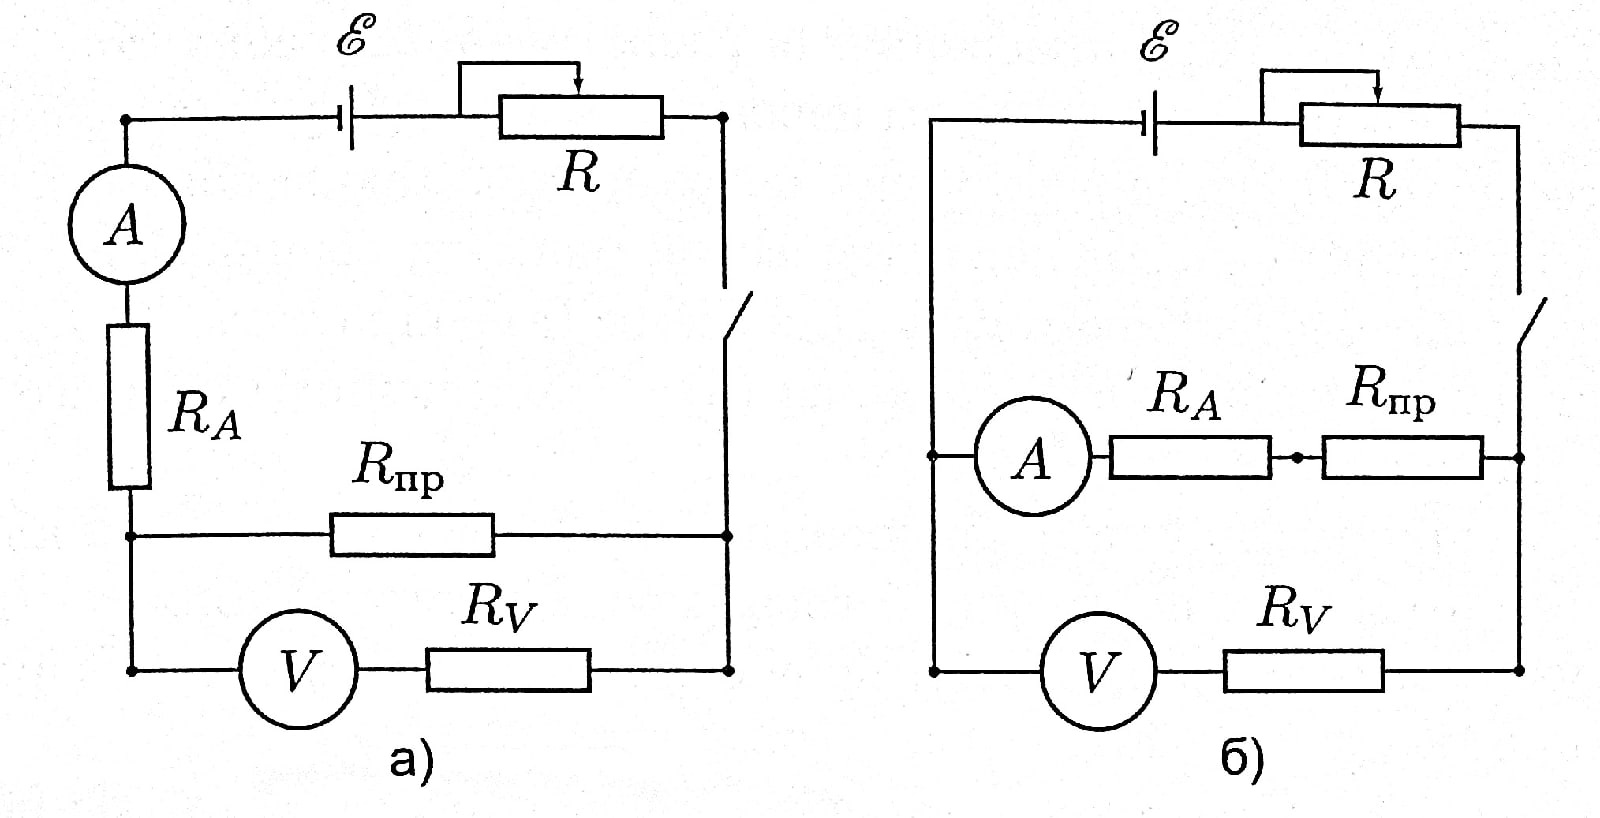
\includegraphics[width=0.8\textwidth]{schemas.jpg}
    \caption{Чертеж схем (a) и (б).}
    \label{pic:schemas}
\end{figure}  

Учтем, что $R_{пр} \approx 5 ~ Oм$, $R_V = 10^7 ~ Ом$, $R_A = 64 \cdot 10^{-3} ~ Ом$. Тогда получим:

для схемы (a): $R_{пр} / R_V = \frac{5}{10^7} = 5 \cdot 10^{-7}$

для схемы (б): $R_{A} / R_{пр} = \frac{64 \cdot 10^{-3}}{5} = 0.0128$

Следовательно, меньшую ошибку дает схема (а).

\point Соберем схему (а).

\point Проведем опыты для проволоки длины $l_1 = (10 \pm 0.1) \quad см$, $l_2 = (20 \pm 0.1) \quad см$, $l_1 = (30 \pm 0.1) \quad см$. Показания вольтметра и амперметра записаны в таблицу \ref{tabl:resitanses}, результаты измерения сопротивлений с помощью моста P4833 записаны в таблицу  \ref{tabl:bridge}.

\begin{table}[!h]
    \centering
    \begin{tabularx}{\textwidth}
        {|C|C||C|C||C|C|}
        \hline
        \multicolumn{2}{|c}{$l_1 = (10 \pm 0.1) \quad см$} & \multicolumn{2}{||c||}{$l_2 = (20 \pm 0.1) \quad см$} & \multicolumn{2}{c|}{$l_3 = (30 \pm 0.1) \quad см$} \\ \hline
        V, В & I, дел ($0.005 \frac{А}{дел}$) & V, В & I, дел ($0.005 \frac{А}{дел}$) & V, В & I, дел ($0.005 \frac{А}{дел}$) \\ \hline
        0.1735 & 33 & 0.3670 & 35 & 0.5510 & 35 \\ \hline
        0.2149 & 40 & 0.4204 & 40 & 0.6390 & 40 \\ \hline
        0.2443 & 45 & 0.4785 & 45 & 0.7215 & 45 \\ \hline
        0.2707 & 50 & 0.5297 & 50 & 0.8122 & 50 \\ \hline
        0.2971 & 55 & 0.5818 & 55 & 0.8800 & 55 \\ \hline
        0.3192 & 60 &   -    & -  & 0.9605 & 60 \\ \hline
    \end{tabularx}
    \caption{Показания вольтметра и амперметра}
    \label{tabl:resitanses}
\end{table}

\begin{table}[!h]
    \centering
    \begin{tabularx}{\textwidth}
        {|C||C||C|}
        \hline
        $l_1 = (10 \pm 0.1) \quad см$ & $l_2 = (20 \pm 0.1) \quad см$ & $l_3 = (30 \pm 0.1) \quad см$ \\ \hline
        $R_{пр} = 1.132 \quad Ом$ & $R_{пр} = 2.208 \quad Ом$ & $R_{пр} = 3.279 \quad Ом$ \\ \hline
    \end{tabularx}
    \caption{Результаты измерения сопротивления проволоки на мосту.}
    \label{tabl:bridge}
\end{table}

\point Построим вольт-амперную характеристику для каждой длины проволоки по таблице \ref{tabl:resitanses} (рис. \ref{pic:graph}). 

\begin{figure}[h!]
    \centering
    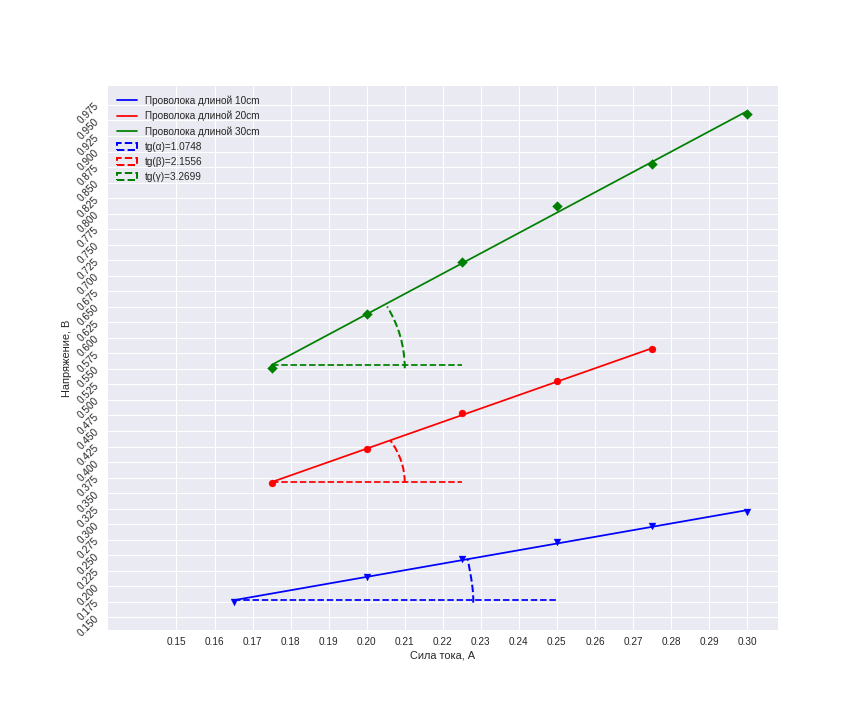
\includegraphics[width=\textwidth]{plot.png}
    \caption{График зависимости тока от напряжения для проволоки}
    \label{pic:graph}
\end{figure}  

\point Из рисунка \ref{pic:graph} определяем $R_{ср}$  -- среднее сопротивление каждой проволки--, найдя тангенс угла наклона каждй прямой. Погрешность $R_{ср}$ определяем по формуле:
\begin{equation} \label{eq:5}
   \sigma_{R_{ср}} =  R_{ср} \sqrt { \left(\frac{\sigma_{V}}{V_{max}}\right)^2 + \left(\frac{\sigma_{I}}{I_{max}}\right)^2 }
\end{equation}

Где 
    $\sigma_{V}$ -- среднеквадратичная ошибка измерения вольтметром,
    $\sigma_{I}$ -- среднеквадратичная ошибка измерения амперметром,
    $V_{max}$ -- максимальное значение напряжения, полученное в эксперименте,
    $I_{max}$ -- максимальное значение силы тока, полученное в эксперименте.

Заметим, что ошибки $\sigma_{V} = \frac{\Delta x}{2} \approx 0.75 \quad мВ$ и  $\sigma_{I} = \frac{\Delta x}{2} \approx 0.4 \quad мА$ равны половине абсолютной погрешности прибора соответственно.

\point Результаты расчетов занесем в таблицу \ref{tabl:pre_results}

\begin{table}[!h]
    \centering
    \begin{tabularx}{\textwidth}
        {|C|C|C|C|}
        \hline
        $l, \quad см$ & 10 & 20 & 30 \\ \hline
        $R_{ср}, \quad Ом$ & 1.0748 & 2.1556 & 3.2699 \\ \hline
        $\sigma_{R_{ср}}, \quad Ом$ & 0.002864 & 0.004111 & 0.005052 \\ \hline
    \end{tabularx}
    \caption{Результаты расчетов средних сопротивлений и их погрешностей из рисунка \ref{pic:graph}.}
    \label{tabl:pre_results}
\end{table}

\point Согласно формуле \eqref{eq:2} найдем окончательное значение сопротивления $R_{пр}$ для каждого участка проволоки. Ввиду малости поправки будем считать, что $\sigma_{R_{пр}} \approx \sigma_{R_{ср}}$. Результаты знаносим в таблицу \ref{tabl:results}.

\begin{table}[!h]
    \centering
    \begin{tabularx}{\textwidth}
        {|C|C|C|C|}
        \hline
        $l, \quad см$ & 10 & 20 & 30 \\ \hline
        $R_{пр}, \quad Ом$ & 1.074800116 & 2.155600456 & 3.269901069 \\ \hline
        $\sigma_{R_{пр}}, \quad Ом$ & 0.002864 & 0.004111 & 0.005052 \\ \hline
    \end{tabularx}
    \caption{Результаты расчетов сопротивлений проволоки и их погрешностей из рисунка \ref{pic:graph}.}
    \label{tabl:results}
\end{table}

\point Сравним результаты из таблицы \ref{tabl:results} с результами измерений мостом Р4833 из таблицы \ref{tabl:resitanses}. Заметим, что с учетом погрешностей эксперимента, результаты совпадают.

\point По формуле \eqref{eq:1} определим удельное сопротивлеие, а погрешность найдем по формуле:

\begin{equation} \label{eq:6}
    \sigma_{\rho} =  \rho \sqrt { \left(\frac{\sigma_{R}}{R}\right)^2 + \left(2 \frac{\sigma_{d}}{d} \right)^2 + \left(\frac{\sigma_{l}}{l} \right)^2}
\end{equation}

Где 
    $\sigma_{R}$ -- ошибка измерения cопротивления,
    $\sigma_{d}$ -- ошибка измерения диаметра проволоки,
    $\sigma_{l}$ -- ошибка измерения длины проволоки,
    $\rho$ -- расчетное значение удельного сопротивления,
    $R$ -- расчетное значение напряжения,
    $d$ -- расчетное значение диаметра проволоки,
    $l$ -- значение длины проволоки.

Результаты занесем в таблицу \ref{tabl:final_results}


\begin{table}[!h]
    \centering
    \begin{tabular}{|c|c|c|c|}
        \hline
        $l, \quad см$ & 10 & 20 & 30 \\ \hline
        $\rho, \quad 10^{-6} ~ Ом \cdot м$ & 1.0879 & 1.0909 & 1.1033 \\ \hline
        $\sigma_{\rho}, \quad 10^{-8} ~ Ом \cdot м$ & 6.164 & 6.054 & 6.159 \\ \hline
    \end{tabular}
    \caption{Результаты расчетов удельного сопротивления проволки}
    \label{tabl:final_results}
\end{table}

Окончательное $\rho = \rho_{ср} = (1.094 \pm 0.0612) \cdot 10^{-6} ~ Ом \cdot м$. 

\parag {Заключение} ~\\
Полученное значение удельного сопротивления хорошо соотносится с табличными значениями. В различных справочниках табличное значение удельного сопротивления нихрома при 20\textdegree{}C варьируется от $1.05 \cdot 10^{-6} ~ Ом \cdot м$ до $1.12 \cdot 10^{-6} ~ Ом \cdot м$, в зависимости от процентного содержания компонент сплава. В конечном счете, это говорит о верности полученных результатов.
\end{document}
